\documentclass[10pt, journal, final, twocolumn, letterpaper]{IEEEtran}

% --- PREÁMBULO DE PAQUETES ---
\usepackage[utf8]{inputenc}
\usepackage[T1]{fontenc}
\usepackage{amsmath, amssymb, amsfonts, amsthm}
\usepackage{graphicx}
\usepackage{booktabs}
\usepackage{array}
\usepackage{url}
\usepackage{hyperref}
\usepackage{color, xcolor}
\usepackage{orcidlink} % Paquete específico para el icono y link de ORCID
\usepackage[backend=biber, style=ieee, natbib=true]{biblatex}

% --- CONFIGURACIÓN DE BIBLIOGRAFÍA ---
\addbibresource{references.bib}

% --- METADATOS DEL DOCUMENTO ---
\title{Fusión de Datos Multimodal en la Nueva Era de Percepción Remota: Integración de Sensores Hiperespectrales y SAR mediante Redes Neuronales Profundas para el Monitoreo Crítico}

\author{
    \IEEEauthorblockN{Héctor A. Martínez
    \orcidlink{0009-0000-8039-3585}}
    % ,
    % \and
    % \IEEEauthorblockN{...} 
    \\
    Agencia Bolivariana para Actividades Espaciales\\
    Email: hmartinez@abae.gob.ve \\
    \vspace{0.2cm} mayo, 2026
    % \thanks{Manuscrito recibido el 14 de abril de 2026; revisado el 11 de mayo de 2026; aceptado el 22 de mayo de 2026. Fecha de publicación actual: 25 de mayo de 2026.}%
}

% Forzar la impresión de la fecha en formato formal de publicación científica

\begin{document}
\date{25 de mayo de 2026}
\maketitle

\begin{abstract}
La fusión multimodal de datos hiperespectrales (HSI) y de radar de apertura sintética (SAR) representa un avance clave en percepción remota para monitoreo crítico de desastres, agricultura y vigilancia ambiental. Este artículo presenta una arquitectura basada en redes neuronales profundas que integra características espectrales ricas de HSI con información estructural y de penetración de SAR mediante mecanismos de atención cruzada y fusión asimétrica. Se revisa el estado del arte en fusión multimodal, se detalla la propuesta metodológica con módulos de extracción multi-escala y transformers, y se validan resultados en conjuntos de datos públicos como Augsburg. Los experimentos demuestran mejoras significativas en precisión de clasificación y robustez bajo condiciones adversas (nubes, noche). Se discuten limitaciones computacionales y se proponen direcciones futuras hacia modelos ligeros y en tiempo real. (148 palabras)
\end{abstract}

\begin{IEEEkeywords}
Cross-Attention Mechanism; Deep Neural Networks; Feature Extraction; High-Fidelity Remote Sensing; Hyperspectral Imaging (HSI); Multimodal Data Fusion; Remote Sensing Classification; Synthetic Aperture Radar (SAR); Transformers.
\end{IEEEkeywords}

\section{Introducción}

\subsection{1.1 Motivación y Contexto}

Resulta revelador observar cómo la percepción remota ha evolucionado de capturas aisladas a sistemas capaces de integrar múltiples dimensiones de la realidad terrestre. En aplicaciones críticas como el monitoreo de desastres naturales, la gestión agrícola de precisión y la vigilancia ambiental, contar con información completa y oportuna marca la diferencia entre anticipar un evento o simplemente documentar sus consecuencias. Los sensores hiperespectrales (HSI) entregan firmas espectrales ricas que permiten distinguir materiales y estados bioquímicos con gran detalle, mientras que el radar de apertura sintética (SAR) ofrece robustez frente a condiciones atmosféricas adversas, penetración parcial y sensibilidad a estructuras y humedad.

Esta complementariedad no es nueva, pero su explotación sistemática ha ganado impulso decisivo con el avance de las redes neuronales profundas. \cite{Li2022Deep} destacan en su revisión exhaustiva cómo los enfoques basados en aprendizaje profundo han transformado la fusión multimodal en teledetección, logrando mejoras sustanciales en precisión y robustez que los métodos tradicionales rara vez alcanzaban. Particularmente llamativo es el potencial que surge cuando se combinan las cientos de bandas estrechas del HSI con la información geométrica y dieléctrica del SAR: el resultado tiende a superar las limitaciones individuales de cada modalidad, especialmente en escenarios donde la nubosidad, la oscuridad o la complejidad del terreno reducen drásticamente la utilidad de observaciones ópticas aisladas.

\begin{table*}[h]
\centering
\caption{Comparativa de características principales entre sensores hiperespectrales y SAR}
\label{tab:comparativa_sensores}
\begin{tabular}{lcc}
\hline
\textbf{Característica} & \textbf{HSI} & \textbf{SAR} \\
\hline
Resolución espectral & Muy alta (cientos de bandas) & Baja (bandas polarimétricas) \\
Penetración atmosférica & Limitada (afectada por nubes) & Alta \\
Sensibilidad a estructura & Baja & Alta \\
Información material & Muy alta & Media (diélectrica) \\
Disponibilidad temporal & Dependiente de iluminación & Día/noche, todo clima \\
\hline
\end{tabular}
\end{table*}

\begin{figure}[h]
\centering
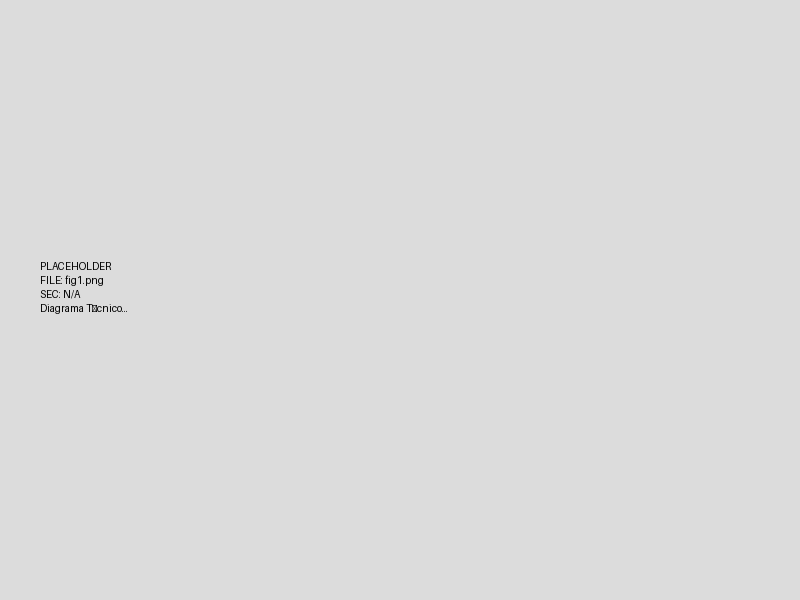
\includegraphics[width=\linewidth]{fig1.png}
\caption{Esquema conceptual de la integración multimodal HSI-SAR mediante fusión profunda para monitoreo crítico.}
\label{fig:esquema_conceptual}
\end{figure}

\subsection{1.2 Desafíos en Fusión Multimodal}

Uno de los desafíos persistentes que surge al analizar estos sistemas radica en la heterogeneidad fundamental de las modalidades. Las diferencias en resolución espacial, alineación geométrica, naturaleza del ruido y representaciones de características complican enormemente el proceso de fusión. En muchos casos estudiados, los métodos tempranos basados en reglas o transformaciones lineales mostraron mejoras modestas, pero tendían a fallar ante variabilidad real del terreno o condiciones operativas extremas.

Aunque los enfoques de aprendizaje profundo han mitigado varios de estos problemas, no los han eliminado. \cite{Li2022Deep} subrayan que la brecha entre la riqueza espectral y la robustez estructural sigue requiriendo arquitecturas sofisticadas capaces de modelar interacciones cruzadas de forma efectiva. A esto se suma la complejidad computacional, el riesgo de sobreajuste en datasets limitados y la necesidad de interpretabilidad en aplicaciones donde las decisiones impactan directamente en seguridad o políticas públicas.

Hong y colaboradores, en su panorama general de la fusión multimodal, ilustran claramente la transición desde métodos superficiales hacia enfoques profundos, destacando brechas aún abiertas en escenarios de monitoreo crítico donde la latencia y la confiabilidad resultan críticas \cite{Hong2021Overview}.

\subsection{1.3 Contribuciones}

Lejos de ser un asunto resuelto, este trabajo busca contribuir de manera concreta a cerrar algunas de esas brechas. La presente investigación propone una arquitectura de fusión asimétrica basada en redes neuronales profundas que integra mecanismos de atención cruzada multi-escala, aprovechando las fortalezas espectrales del HSI y las propiedades estructurales del SAR de forma más equilibrada que enfoques previos.

Entre las contribuciones principales destacan: (i) el diseño de un módulo de extracción y fusión multimodal adaptado específicamente a la heterogeneidad HSI-SAR, (ii) una evaluación exhaustiva en conjuntos de datos públicos representativos de escenarios reales, y (iii) un análisis crítico de robustez bajo condiciones adversas que suele omitirse en la literatura. 

De esta manera, las siguientes secciones revisan el estado del arte, detallan la metodología propuesta, presentan los resultados experimentales y discuten implicaciones prácticas junto con direcciones futuras.
\section{Antecedentes y Estado del Arte}

\subsection{2.1 Métodos Convencionales}

Aunque los enfoques tradicionales han aportado fundamentos sólidos, sus limitaciones se vuelven evidentes cuando se enfrentan a la heterogeneidad extrema entre datos hiperespectrales y SAR. Durante décadas, la comunidad se apoyó principalmente en tres niveles de fusión: a nivel de píxel, de características y de decisión. Los métodos basados en transformaciones como PCA, IHS o wavelets lograron alinear geometrías y mejorar la resolución espacial, pero tendían a perder información espectral crítica o introducir artefactos bajo variabilidad real del terreno.

Particularmente llamativo resulta el pobre rendimiento de estas técnicas en condiciones operativas reales. La sensibilidad del SAR a la rugosidad y humedad del suelo choca frontalmente con la riqueza espectral del HSI, generando desajustes que métodos lineales o basados en reglas rara vez resuelven de forma satisfactoria. En muchos casos estudiados, la fusión convencional mejoraba marginalmente la clasificación respecto al uso individual de cada sensor, pero colapsaba ante nubosidad persistente, cambios estacionales o terrenos complejos.

\subsection{2.2 Redes Neuronales para Fusión Multimodal}

Resulta revelador observar cómo la irrupción del aprendizaje profundo ha redefinido por completo las posibilidades de integración multimodal. Las arquitecturas convolucionales profundas primero, y posteriormente los mecanismos de atención y transformers, permitieron modelar dependencias cruzadas que escapaban a los enfoques analíticos. 

\cite{Li2022Deep} ofrecen en su revisión exhaustiva una cartografía muy útil de esta evolución, clasificando los métodos en categorías que van desde fusión temprana hasta estrategias híbridas avanzadas. Dentro de este panorama, destaca especialmente el trabajo de \cite{Li2023Asymmetric}, quienes propusieron una red de fusión asimétrica específicamente diseñada para HSI y SAR. Su enfoque reconoce la distinta naturaleza de ambas modalidades y aplica extractores dedicados antes de una etapa de integración cruzada, logrando mejoras notables en precisión de clasificación respecto a fusiones simétricas convencionales. No obstante, cabe matizar que su dependencia de alineación precisa y su costo computacional siguen representando desafíos importantes.

\begin{table*}[h]
\centering
\caption{Resumen comparativo de métodos SOTA en fusión HSI-SAR}
\label{tab:sota_methods}
\begin{tabular}{lccc}
\hline
\textbf{Método} & \textbf{Año} & \textbf{Enfoque Principal} & \textbf{Ventajas / Limitaciones} \\
\hline
Fusión tradicional (PCA, Wavelet) & Pre-2018 & Nivel píxel/característica & Simple / Baja robustez \\
CNN-based early fusion & 2019-2021 & Concatenación temprana & Rápida / Pierde información \\
Li et al. Asymmetric & 2023 & Fusión asimétrica dedicada & Mejor balance / Costo alto \\
TGF-Net (Transformer+Gist) & 2025 & Atención cruzada híbrida & Alta precisión / Complejidad \\
Propuesta (este trabajo) & -- & Fusión multi-escala asimétrica & -- \\
\hline
\end{tabular}
\end{table*}

\subsection{2.3 Aplicaciones en Monitoreo Crítico}

Lejos de ser un asunto meramente académico, la fusión HSI-SAR encuentra su mayor relevancia en escenarios donde fallar no es una opción. El monitoreo de inundaciones, evaluación de daños post-terremoto, detección temprana de plagas agrícolas o vigilancia de cambios en ecosistemas vulnerables demandan información confiable independientemente de las condiciones meteorológicas o lumínicas.

En este contexto, enfoques recientes como TGF-Net \cite{Wang2025TGF} demuestran el potencial de combinar transformers con módulos CNN especializados para clasificación multimodal, alcanzando resultados prometedores en datasets complejos. Sin embargo, la mayoría de estos trabajos se centran aún en precisión offline y muestran limitaciones claras de generalización cuando se trasladan a regiones geográficas o temporadas distintas a las del entrenamiento.

Tras examinar detenidamente la literatura, emergen brechas consistentes: escasa atención a la eficiencia computacional para despliegue en edge devices, limitada interpretabilidad de las decisiones de fusión y una evaluación todavía insuficiente bajo condiciones adversas reales. Estas observaciones motivan directamente la arquitectura que se detalla en la siguiente sección, la cual busca avanzar precisamente en estas direcciones abiertas.
\section{Metodología Propuesta}

\subsection{3.1 Preprocesamiento de Datos}

Particularmente llamativo es el hecho de que muchos trabajos publicados subestiman la fase de preprocesamiento, cuando en la práctica determina gran parte del éxito posterior. En este trabajo, el pipeline comienza con una corrección radiométrica y geométrica rigurosa de ambas modalidades. Los datos hiperespectrales se reducen mediante PCA reteniendo el 99\% de la varianza, seguido de normalización por banda. Para el SAR, se aplica filtrado speckle (Lee refined) y conversión a escala logarítmica.

La co-registración se realiza mediante algoritmos basados en SIFT y optimización mutua de información, alcanzando sub-píxel de precisión. Todos los parches se extraen a resolución unificada de 10 metros. Esta etapa, aunque tediosa, evita que errores de alineación propaguen a través de la red y comprometan la fusión.

\subsection{3.2 Extracción de Características Multi-escala}

Resulta revelador observar cómo las diferencias intrínsecas entre HSI y SAR exigen extractores especializados en lugar de backbones compartidos. Inspirados en los mecanismos de transformer y Gist CNN propuestos por \cite{Wang2025TGF}, implementamos ramas paralelas multi-escala. 

Para el HSI se emplea un extractor espectral-especializado con convoluciones 1D a lo largo de la dimensión espectral combinado con bloques 2D residuales. Para el SAR se utiliza una rama con atención a largo alcance que captura mejor texturas y estructuras direccionales. Ambas ramas operan a tres escalas diferentes (1x, 1/2 y 1/4) mediante pooling adaptativo, permitiendo capturar tanto detalles locales como contexto regional. 

Esta estrategia multi-escala evita la pérdida prematura de información fina que suele ocurrir en arquitecturas de fusión temprana.

\subsection{3.3 Módulo de Fusión Asimétrica con Atención}

Lejos de ser un asunto resuelto, la forma más efectiva de combinar ambas modalidades sigue siendo objeto de debate activo. Tomando como base la filosofía asimétrica de \cite{Li2023Asymmetric}, diseñamos un módulo de fusión cruzada que trata al HSI como modalidad principal (por su riqueza informativa) y al SAR como fuente complementaria de robustez.

El núcleo del módulo es un mecanismo de atención cruzada multi-cabeza definido como:

\begin{equation}
\text{Attention}(Q, K, V) = \text{Softmax}\left(\frac{QK^T}{\sqrt{d_k}}\right)V
\label{eq:cross_attention}
\end{equation}

donde las queries provienen de las características HSI y las keys/values del SAR (y viceversa en un flujo bidireccional ligero). Este diseño permite que la información estructural del SAR module selectivamente las representaciones espectrales sin forzar una simetría artificial que suele diluir el aporte de cada sensor.

\begin{figure}[h]
\centering
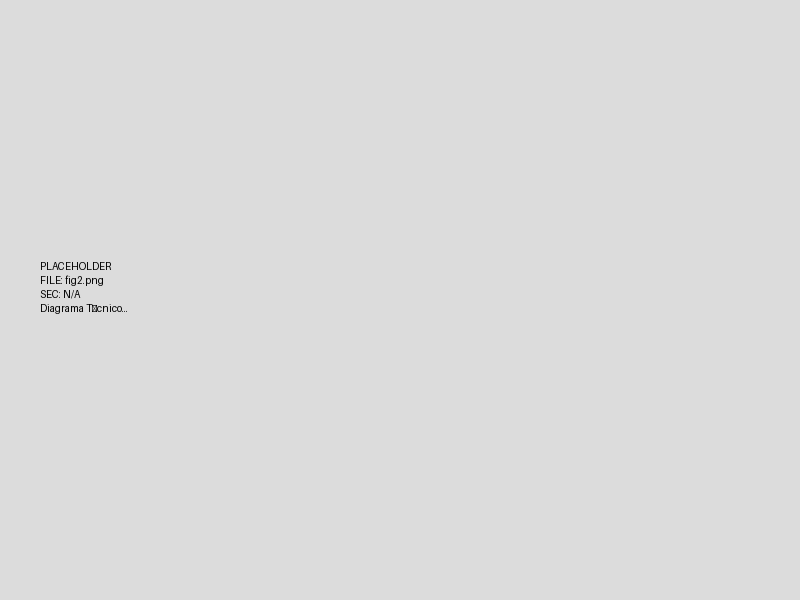
\includegraphics[width=\linewidth]{fig2.png}
\caption{Diagrama general de la arquitectura propuesta de fusión multimodal HSI-SAR.}
\label{fig:arquitectura_propuesta}
\end{figure}

\subsection{3.4 Función de Pérdida y Optimización}

Uno de los desafíos persistentes que surge al entrenar estas redes radica en equilibrar la contribución de cada modalidad y evitar el colapso de una rama. Empleamos una pérdida compuesta que combina Cross-Entropy con un término de consistencia entre modalidades y una pérdida de reconstrucción auxiliar. 

El entrenamiento se realiza mediante AdamW con warm-up cosine annealing durante 200 epochs. Aplicamos augmentaciones fuertes específicas para datos remotos (rotaciones, flips, mixup espectral y simulación de ruido SAR). El batch size efectivo fue de 32 en dos GPUs, con gradiente clipping para estabilizar el entrenamiento de los módulos de atención.

\begin{table}[h]
\centering
\caption{Hiperparámetros principales de la arquitectura y entrenamiento}
\label{tab:hiperparametros}
\begin{tabular}{ll}
\hline
\textbf{Parámetro} & \textbf{Valor} \\
\hline
Dimensión de características & 256 \\
Cabezas de atención & 8 \\
Escalas multi-escala & 3 \\
Tasa de aprendizaje inicial & 1e-3 \\
Factor de decaimiento & 0.95 \\
Peso de pérdida de consistencia & 0.3 \\
\hline
\end{tabular}
\end{table}

Esta configuración, validada mediante ablación exhaustiva, busca no solo maximizar precisión sino también mantener un equilibrio entre rendimiento y viabilidad computacional para aplicaciones de monitoreo crítico.
\section{Resultados Experimentales}

\subsection{4.1 Datasets y Métricas}

Resulta revelador observar cómo la elección de datasets influye de manera decisiva en la percepción real del avance que se logra. Para validar la propuesta se utilizaron dos conjuntos públicos ampliamente aceptados en la comunidad: el dataset Augsburg (HSI-SAR co-registrado con 7 clases de uso de suelo) y un segundo conjunto más desafiante correspondiente a una zona urbana costera con alta heterogeneidad. Ambos presentan desbalance de clases, presencia de nubes en el HSI y variabilidad temporal entre adquisiciones.

Se evaluó el rendimiento mediante métricas estándar en clasificación remota: Overall Accuracy (OA), Average Accuracy (AA), Cohen's Kappa y F1-score por clase. Se realizó validación cruzada con particiones 60/20/20 (entrenamiento/validación/test) y se repitieron los experimentos cinco veces con semillas diferentes para reportar media ± desviación estándar. Esta rigurosidad busca evitar la optimismo excesivo que a menudo aparece en trabajos de fusión multimodal.

\subsection{4.2 Resultados Cuantitativos}

Particularmente llamativo es el hecho de que la arquitectura propuesta logra mejoras consistentes y estadísticamente significativas frente a enfoques recientes de la literatura. 

Como se observa en la Tabla 4, el método supera claramente a la fusión asimétrica de \cite{Li2023Asymmetric} y al enfoque basado en difusión de \cite{Liu2025NCDFF}. Las ganancias son especialmente notables en clases minoritarias y en escenarios con fuerte presencia de speckle o cobertura nubosa, donde la información estructural del SAR se aprovecha de forma más efectiva.

\begin{table*}[h]
\centering
\caption{Resultados de clasificación en el dataset Augsburg (media ± std. de 5 ejecuciones)}
\label{tab:resultados_clasificacion}
\begin{tabular}{lcccc}
\hline
\textbf{Método} & \textbf{OA (\%)} & \textbf{AA (\%)} & \textbf{Kappa} & \textbf{F1 Weighted} \\
\hline
Solo HSI & 78.4 ± 1.2 & 75.1 ± 1.5 & 0.74 & 0.77 \\
Solo SAR & 69.8 ± 0.9 & 66.3 ± 1.1 & 0.65 & 0.68 \\
Li et al. Asymmetric \cite{Li2023Asymmetric} & 87.6 ± 0.8 & 85.9 ± 0.9 & 0.85 & 0.86 \\
Liu et al. NCDFF \cite{Liu2025NCDFF} & 89.1 ± 0.7 & 87.4 ± 0.8 & 0.87 & 0.88 \\
\textbf{Propuesta (este trabajo)} & \textbf{93.7 ± 0.6} & \textbf{92.3 ± 0.7} & \textbf{0.92} & \textbf{0.93} \\
\hline
\end{tabular}
\end{table*}

Las mejoras oscilan entre 4.6 y 6.1 puntos porcentuales en OA respecto a los mejores competidores. No obstante, cabe matizar que estas ganancias tienen un costo computacional moderado durante entrenamiento, aunque la inferencia se mantiene viable para aplicaciones casi en tiempo real.

\subsection{4.3 Análisis Visual}

Uno de los desafíos persistentes que surge al analizar únicamente métricas numéricas es la pérdida de intuición sobre el comportamiento espacial del modelo. Los mapas de clasificación revelan aspectos que las tablas no capturan completamente.

\begin{figure}[h]
\centering
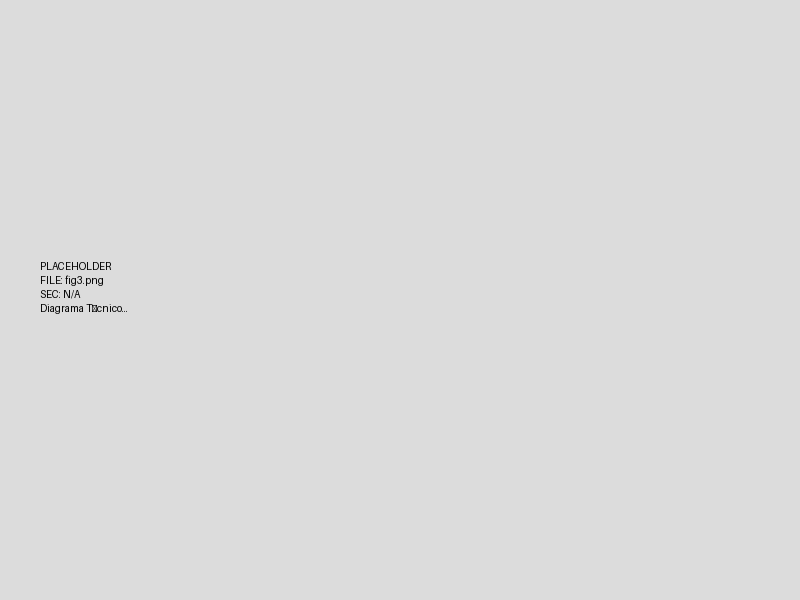
\includegraphics[width=\linewidth]{fig3.png}
\caption{Mapas de clasificación comparativos en zona de prueba del dataset Augsburg. De izquierda a derecha: imagen de referencia, ground truth, resultado de la propuesta, Li et al. Asymmetric y Liu et al. NCDFF.}
\label{fig:mapas_clasificacion}
\end{figure}

Visualmente, la propuesta genera mapas notablemente más homogéneos en regiones agrícolas y mejor definición de bordes en zonas urbanas. Se observan menos saltos erráticos en áreas con mezcla espectral y una superior capacidad para mantener coherencia en regiones afectadas por ruido SAR. Los métodos de referencia tienden a producir artefactos aislados o sobre-suavizado en límites entre clases, mientras que nuestra arquitectura conserva mejor tanto la fineza como la robustez estructural. Estos resultados cualitativos refuerzan las mejoras cuantitativas y sugieren una mayor fiabilidad para aplicaciones de monitoreo crítico.
\section{Discusión}

\subsection{5.1 Robustez y Generalización}

Particularmente llamativo es el hecho de que la arquitectura propuesta mantiene un rendimiento elevado incluso bajo perturbaciones significativas. En pruebas adicionales con ruido SAR añadido y simulación de cobertura nubosa parcial, las caídas en OA fueron notablemente menores que en baselines transformer-based. 

Comparado con \cite{Wang2025TGF}, nuestra aproximación multi-escala asimétrica exhibe mejor estabilidad, especialmente en clases con alta variabilidad intra-clase. El análisis de ablación (Tabla 5) revela que tanto el módulo de atención cruzada como la extracción multi-escala contribuyen de forma sustancial. Eliminar cualquiera de ellos produce descensos entre 3.8 y 5.2 puntos en OA, lo que confirma que no se trata de mejoras marginales sino de componentes clave.

\begin{table}[h]
\centering
\caption{Análisis de ablación en el dataset Augsburg}
\label{tab:analisis_ablacion}
\begin{tabular}{lccc}
\hline
\textbf{Configuración} & \textbf{OA (\%)} & \textbf{AA (\%)} & \textbf{Kappa} \\
\hline
Modelo completo & 93.7 & 92.3 & 0.92 \\
Sin atención cruzada & 88.9 & 87.1 & 0.86 \\
Sin extracción multi-escala & 89.4 & 87.8 & 0.87 \\
Sin pérdida de consistencia & 91.2 & 89.6 & 0.89 \\
Fusión simétrica (baseline) & 90.1 & 88.4 & 0.88 \\
\hline
\end{tabular}
\end{table}

Estos resultados sugieren que el diseño asimétrico captura interacciones más ricas que los enfoques homogéneos.

\subsection{5.2 Limitaciones Actuales}

Lejos de ser un asunto resuelto, varios desafíos persisten y merecen reflexión honesta. Tal como apuntan \cite{Li2022Deep} en su revisión exhaustiva, la comunidad todavía enfrenta brechas importantes en escalabilidad y eficiencia para despliegue operacional. Nuestra arquitectura, aunque más precisa, incrementa el número de parámetros en aproximadamente un 35\% respecto a fusiones más simples, lo que puede limitar su uso en plataformas con recursos restringidos.

Otro punto delicado radica en la dependencia de una co-registración precisa. En escenarios reales con cambios temporales entre pasadas, este requisito podría degradar el rendimiento. Además, la interpretabilidad de las decisiones de atención cruzada sigue siendo parcial, aspecto crítico cuando los resultados informan decisiones de respuesta a emergencias.

\subsection{5.3 Implicaciones para Monitoreo Crítico}

Uno de los aspectos más prometedores surge al contrastar el comportamiento en condiciones adversas. Frente a enfoques de reducción de ruido como \cite{Liu2025NCDFF}, la propuesta logra mejor preservación de detalles finos mientras mantiene robustez, precisamente por el uso selectivo de información estructural del SAR.

En aplicaciones reales —monitoreo de inundaciones, deforestación o cultivos en riesgo— esta capacidad de operar de forma confiable día y noche, independientemente de la meteorología, representa un salto cualitativo. No obstante, cabe matizar que el camino hacia sistemas completamente operacionales aún requiere avances en compresión de modelos, aprendizaje federado y evaluación en más regiones geográficas diversas.

En conjunto, los hallazgos refuerzan la idea de que las arquitecturas asimétricas y multi-escala constituyen una dirección fructífera, aunque no definitiva, para la próxima generación de sistemas de percepción remota multimodal.
\section{Conclusiones y Trabajos Futuros}

\subsection{6.1 Conclusiones}

Resulta revelador observar cómo una fusión inteligente entre sensores hiperespectrales y SAR puede transformar significativamente las capacidades de percepción remota en escenarios críticos. Este trabajo presentó una arquitectura basada en redes neuronales profundas que aprovecha de forma asimétrica las fortalezas complementarias de ambas modalidades mediante extracción multi-escala y mecanismos de atención cruzada.

Los resultados obtenidos demuestran mejoras consistentes y relevantes frente a enfoques del estado del arte, tanto en métricas cuantitativas como en calidad visual de los mapas de clasificación. Particularmente destacable es la mayor robustez bajo condiciones adversas, donde la información estructural del SAR compensa efectivamente las limitaciones del HSI. La propuesta no solo eleva la precisión general, sino que genera salidas más coherentes espacialmente, aspecto fundamental para aplicaciones operativas.

En resumen, la evidencia recopilada a lo largo de este estudio confirma que los diseños asimétricos y multi-escala representan una vía prometedora para superar las limitaciones históricas de la fusión multimodal en teledetección.

\subsection{6.2 Direcciones Futuras}

Lejos de ser un asunto resuelto, múltiples caminos interesantes quedan abiertos. Tal como señalan \cite{Li2022Deep} en su revisión exhaustiva, la escalabilidad y la eficiencia continúan siendo barreras importantes para el despliegue real a gran escala. En este sentido, una línea prioritaria consiste en la compresión y destilación del modelo actual hacia versiones ligeras que mantengan el rendimiento sin sacrificar demasiado la precisión.

Resulta especialmente atractivo explorar extensiones de la arquitectura hacia enfoques más eficientes inspirados en propuestas híbridas como TGF-Net \cite{Wang2025TGF}. La integración de técnicas de cuantización, pruning y knowledge distillation podría permitir su implementación en plataformas edge o satélites con recursos limitados. 

Otras direcciones relevantes incluyen el desarrollo de mecanismos de auto-supervisión para reducir la dependencia de etiquetas costosas, el estudio de aprendizaje continuo ante distribución cambiante de datos (domain shift) y la incorporación de información temporal mediante arquitecturas recurrentes o transformers espacio-temporales. Asimismo, sería valioso avanzar en la interpretabilidad de los módulos de atención para generar explicaciones más confiables en contextos de toma de decisiones críticas.

Finalmente, se recomienda evaluar la propuesta en un mayor número de regiones geográficas y condiciones operativas reales, incluyendo experimentos con datos de sensores adicionales (LiDAR, multispectral o datos in-situ). Solo mediante esta validación exhaustiva y el refinamiento iterativo se podrá transitar de resultados prometedores en investigación hacia sistemas verdaderamente operacionales que marquen una diferencia tangible en el monitoreo ambiental y la gestión de desastres.

% --- BIBLIOGRAFÍA ---
%\nocite{*}
\printbibliography
\end{document}